% !TEX root = ./Vorlesungsmitschrift AGLA 2.tex 
\chapter{Affine Geometrie}
\lecture{Di 21.04. 10:15}{}
\section{Was ist ein affiner Raum?}
\begin{beispiel}[aus der \agla{1}]
    \( \reals^2, \reals^3 \). 
    In diesen Räumen gibt es einen ausgezeichneten \enquote{Usprung}.
\end{beispiel}
\begin{frage*}
    Wie könne wir eine affine Ebene / affine Räume modellieren, wobei alle Punkte gleichberechtigt sind?
\end{frage*}
\begin{idee*}
    Verwende affine Unterräume.
\end{idee*}
\begin{beispiel}\label{affiner_unterraum}
    Sei \( K \) ein Körper, \( V \) ein \( K \)-Vektorraum, \( W\subseteq V \) ein Untervektorraum und \( v\in V \). 
    Wir nennen \( X=v+W \) einen affinen Unterraum von \( V \). 
    \( X \) ist im Allgemeinen selbst kein Vektorraum unter der Addition in \( V \), aber \( W \) \enquote{operiert} auf \( X \).
    \begin{figure}[H]
        \centering
        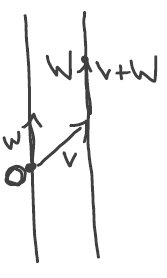
\includegraphics[width=0.2\linewidth]{figures/affiner_unterraum}
        \label{fig:affiner_unterraum}
    \end{figure}
    
    Für \( w\in W \) definieren wir die Abbildung
    \begin{align*}
        \tau_w\maps \begin{aligned}[t] 
            X&\to X\\
            p &\mapsto p+w.
        \end{aligned}
    \end{align*}
    \begin{figure}[H]
        \centering
        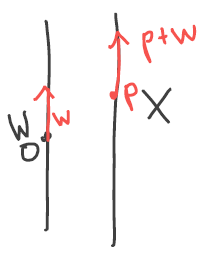
\includegraphics[width=0.2\linewidth]{figures/tau_w}
        \label{fig:tau_w}
    \end{figure}
    Sei
    \begin{align*}
        \bijections{X}=\Set{f\maps X\to X, f \text{ ist bijektiv}}.
    \end{align*}
    Dann ist \( \tau_w\in \bijections{X} \) für alle \( w\in W \).
\end{beispiel}
\begin{bemerkung*}
    \( \bijections{X} \) ist eine Gruppe unter Verkettung von Abbildung. 
    Wir erhalten eine Abbildung
    \begin{align*}
        \tau\maps \begin{aligned}[t] 
            W &\to \bijections{X}\\
            w &\mapsto \tau_w.
        \end{aligned}
    \end{align*}
\end{bemerkung*}
\begin{lemma}
    Die Abbildung \( \tau \) ist ein Gruppenhomomorphismus.
\end{lemma}
\begin{proof}
    Seien \( w, w' \in W \)
    Dann
    \begin{align*}
        \tau_w\circ \tau_{w'}\maps \begin{aligned}[t] 
            X &\to X\\
            p &\mapsto p+\underbracket{w'+w},
        \end{aligned}
    \end{align*}
    also
    \begin{align*}
        \tau(w)\circ \tau(w')=\tau_w\circ \tau_{w'}=\tau_{w+w'}=\tau(w+w').
    \end{align*}
    
\end{proof}
Es gilt noch mehr:

\textcolor{Turquoise}{für \( p, q \in X \)} besteht genau ein \( w\in W \) mit \( \tau_w(p)=q \).

\begin{figure}[H]
    \centering
    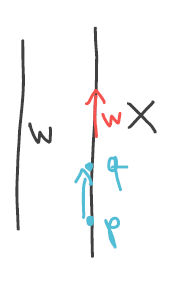
\includegraphics[width=0.2\linewidth]{figures/tau_w_bijektion}
    \label{fig:tau_w_bijektion}
\end{figure}

\subsection*{Gruppenoperationen}
\begin{beispiel}\label{d_3}
    Betrachte ein gleichseitiges Dreieck \( D \) und Spiegelungen / Drehungen die \( D \) auf sich selbst abbilden.

    \begin{figure}[H]
        \centering
        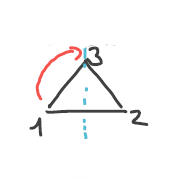
\includegraphics[width=0.2\linewidth]{figures/d_3}
        \label{fig:d_3}
    \end{figure}
    Diese formen eine Gruppe (welche?) und \enquote{operieren} auf \( D \).
\end{beispiel}
\begin{definition}
    Sei \( X \) eine Menge und \( G \) eine Gruppe. 
    Eine Operation von \( G \) auf \( X \) ist ein Homomorphismus von Gruppen
    \begin{align*}
        \tau\maps \begin{aligned}[t] 
            G&\to \bijections{X}\\
            g&\mapsto \tau_g.
        \end{aligned}
    \end{align*}
\end{definition}
\begin{bemerkung*}
    \( \tau \) ist ein Homomorphismus \dh \tforall \( g, g' \in G \)
    \begin{align*}
        \tau_g\circ \tau_{g'}=\tau_{gg'}.
    \end{align*}
    
    Für \( x\in X \) nennen wir
    \begin{align*}
        G(x)=\Set{\tau_g(x)|g\in G}
    \end{align*}
    die Bahn von \( x \) unter \( G \).
\end{bemerkung*}
\begin{beispiel}\label{operation:beispiele}
    \begin{enumerate}
        \item \label{operation:beispiele:linkstranslation} Sei \( G \) eine Gruppe und \( X=G \) die Linkstranslation \( l\maps \begin{aligned}[t] 
            G&\to \bijections{G}\\
            g&\mapsto l_g
        \end{aligned} \) mit \( l_g(x)=gx \quad\forall x\in G \) ist eine Gruppenoperation von \( G \) auf sich selbst.
        
        \item \label{operation:beispiele:konjugation}\begin{align*}
            k\maps \begin{aligned}[t] 
                G &\to \bijections{G}\\
                g &\mapsto k_g
            \end{aligned}
        \end{align*}
        mit \( k_g(x)=gx\inv{g} \quad\forall x\in G \) ist eine Gruppenoperation.
    \end{enumerate}
\end{beispiel}
\begin{frage*}
    Sei \( \tau\maps G\to \bijections{X} \) eine Gruppenoperation, \( x,y\in X \). 
    Wann gibt es ein \( g\in G \) mit \( \tau_g(x)=y \)?
    \begin{figure}[H]
        \centering
        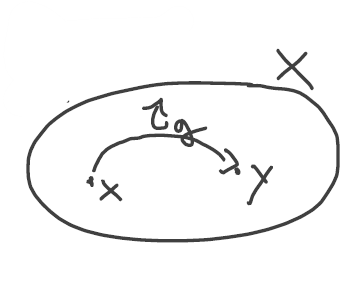
\includegraphics[width=0.5\linewidth]{figures/einfach_transitiv}
        \label{fig:einfach_transitiv}
    \end{figure}
    
\end{frage*}

\begin{definition*}
    Sei \( \tau\maps G\to \bijections{X} \) eine Gruppenoperation von \( G \) auf \( X \). 
    Wir nennen \( \tau \) \emph{einfach transitiv}, wenn \tforall \( x,y\in X \) \emph{genau ein} \( g\in G \) besteht mit
    \begin{align*}
        \tau_g(x)=y.
    \end{align*}
\end{definition*}
\begin{beispiel*}
    \begin{itemize}
        \item Die Gruppenoperation aus \thref{d_3} ist \emph{nicht} einfach transitiv
        \begin{figure}[H]
            \centering
            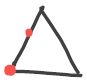
\includegraphics[width=0.2\linewidth]{figures/d_3_nicht_einfach_transitiv}
            \label{fig:d_3_nicht_einfach_transitiv}
        \end{figure}
        
        \item Die Linkstranslation aus \thref{operation:beispiele}~\ref{operation:beispiele:linkstranslation} ist immer einfach transitiv.
    \end{itemize}
\end{beispiel*}
Zurück zum \thref{affiner_unterraum} (\( V \) \( K \)-Vektorraum, \( W\subseteq V \) Untervektorraum, \( v\in V \), \( X=v+W \))

Wir haben Translationen definiert
\begin{align*}
    \tau\maps \begin{aligned}[t] 
        W&\to \bijections{X}\\
        x&\mapsto \tau_w
    \end{aligned}
\end{align*}
mit \( \tau_w\maps X\to X \), \( p\mapsto p+w \). 
\( \tau \) ist eine einfach transitive Gruppenoperation von \( W \) auf \( x \).

\begin{figure}[H]
    \centering
    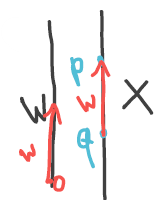
\includegraphics[width=0.2\linewidth]{figures/affiner_unterraum_einfach_transitive_gruppenoperation}
    \label{fig:affiner_unterraum_einfach_transitive_gruppenoperation}
\end{figure}

\begin{definition*}
    Sei \( K \) ein Körper. 
    Ein affiner Raum über \( K \) ist ein Tripel \( (X, T(X), \tau ) \) mit
    \begin{itemize}
        \item \( X\neq \emptyset \) eine Menge 
        \item \( T(X) \) ein \( K \)-Vektorraum 
        \item \( \tau\maps T(x)\to \bijections{X} \) eine einfach transitive Gruppenoperation
    \end{itemize}
\end{definition*}
\begin{konvention*}
    \( X=\emptyset \) ohne Spezifikation von \( T(X) \), \( \tau \) nennen wir auch einen affinen Raum.
\end{konvention*}
\begin{figure}[H]
    \centering
    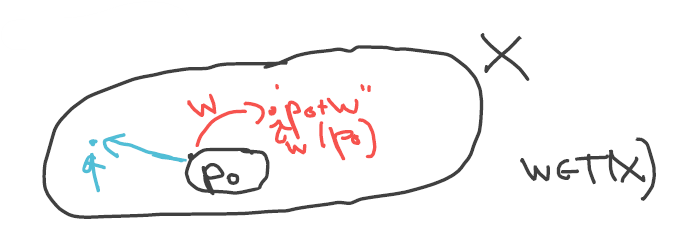
\includegraphics[width=0.5\linewidth]{figures/affiner_raum}
    \label{fig:affiner_raum}
\end{figure}
\begin{definition*}
    Sei \( (X,T(X),\tau) \) in affiner Raum über einem Körper \( K \). 
    Dann nennen wir \( \dim-{K}{T(X)} \) die Dimension von \( X \), schreiben auch \( \affindim-{X} \).
     
    Ist \( \affindim-{X}=1 \) \bzw \( \affindim{X}=2 \), dann nennen wir \( X \) eine affine Gerade \bzw affine Ebene.
\end{definition*}

Sei \( (X, T(X), \tau) \) in affiner Raum, \( p,q\in X \). Dann \( \existsone t\in T(X) \) mit \( \tau_t(p)=q \).

\textcolor{Turquoise}{Schreibe \( \vv{pq}=t\in T(X) \) als \( \tau_{\vv{pq}}(p)=q \).}
\begin{figure}[H]
    \centering
    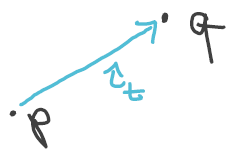
\includegraphics[width=0.2\linewidth]{figures/vektornotation}
    \label{fig:vektornotation}
\end{figure}
Wir erhalten eine Abbildung
\begin{align*}
    X\times X&\to T(X)\\
    (p,q)&\mapsto \vv{pq}.
\end{align*}
\begin{frage*}
    Welche Eigenschaften hat die Abbildung \( (p,q)\mapsto \vv{pq} \) in einem allgemeinen affinen Raum?
\end{frage*}
\begin{lemma}\label{vektoren_funzen_richtig}
    Sei \( X \) ein affiner Raum, \( p,q,r\in X \). Dann gilt \( \vv{pq}+\vv{qr}=\vv{pr} \).
\end{lemma}
\begin{figure}[H]
    \centering
    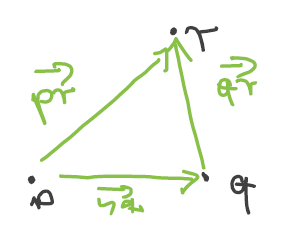
\includegraphics[width=0.3\linewidth]{figures/vektoren_funzen_richtig}
    \label{fig:vektoren_funzen_richtig}
\end{figure}
\begin{proof}
    \( \tau\maps T(X)\to \bijections{X} \) ist ein Homomorphismus. 
    Also gilt \( \tau_{\vv{qr}}\circ \tau_{\vv{pq}}=\tau_{\vv{pq}+\vv{qr}} \). 
    Es gilt damit \( \tau_{\vv{pq}+\vv{qr}}(p)=r \). 
    Also \( \vv{pq}+\vv{qr}=\vv{pr} \).    
\end{proof}

\section{Affine Abbildungen}
Seien \( V,W \) \( K \)-Vektorräume.
In der \agla{1}: lineare Abbildungen
\begin{align*}
    F\maps V\to W,
\end{align*}
\dh \( F \) respektiert die Vektorraum-Struktur
\begin{align*}
    F(v_1+v_2)=F(v_1)+F(v_2)\quad\forall v_1,v_2\in V\\
    F(\lambda v)=\lambda F(v)\quad \forall\lambda\in K \forall v \in V.
\end{align*}
\begin{frage*}
    Was sind natürliche Abbildungen zwischen affinen Räumen?
\end{frage*}
Seien \( X, Y \) affine Räume über einem Körper \( K \).
\begin{figure}[H]
    \centering
    \includegraphics[width=0.8\linewidth]{figures/affine_Abbildungen}
    \label{fig:affine_Abbildungen}
\end{figure}
\begin{align*}
    \textcolor{Turquoise}{\underrelate{\vertni}{T(X)}{\vv{pq}}\rightsquigarrow\underrelate{\vertni}{T(Y)}{\vv{f(p)f(q)}}}.
\end{align*}
\begin{definition*}
    Wir nennen eine Abbildung \( f\maps X \to Y \) affin, wenn es eine \( K \)-lineare Abbildung \( F\maps T(X)\to T(Y) \) gibt, sodass \tforall \( p,q\in X \) gilt
    \begin{align*}
        \vv{f(p)f(q)}=F(\vv{pq}).
    \end{align*}
\end{definition*}
\begin{bemerkung*}
    \begin{enumerate}
        \item Es gibt im Allgemeinen verschiedene affine Abbildungen \( f\maps X \to Y \), die zur gleichen linearen Abbildung \( F\maps T(X)\to T(Y) \) gehören.
        \item Sei \( p_0 \in X \) fest und \( f\maps X \to Y \) affin.
        
        Für \( q\in X \) gilt
        \begin{align*}
            f(q)\begin{aligned}[t] 
                &=\tau_{\vv{f(p_0)f(q)}}(f(p0))\\
            &=\tau_{F(\vv{p_0 q})}(f(p0)).
            \end{aligned}
        \end{align*}
        Also bestimmen \( f(p_0) \) und \( F \) zusammen die Abbildung \( f\maps X\to Y \).
    \end{enumerate}


\end{bemerkung*}
\begin{beispiel*}
    Seien \( V,W \) \( K \)-Vektorräume
    \begin{align*}
        X=(V,V,\tau),\quad Y=(W,W,\tau).
    \end{align*}
    Eine affine Abbildung \( f\maps V\to W \) ist eindeutig bestimmt durch \( f(0) \) und eine lineare Abbildung \( F\maps V\to W \). Es gilt
    \begin{align*}
        f(v)=\textcolor{Goldenrod}{f(0)}+\textcolor{LimeGreen}{F(v)}\quad\forall \textcolor{LimeGreen}{v} \in V.
    \end{align*}
\end{beispiel*}
\begin{figure}[H]
    \centering
    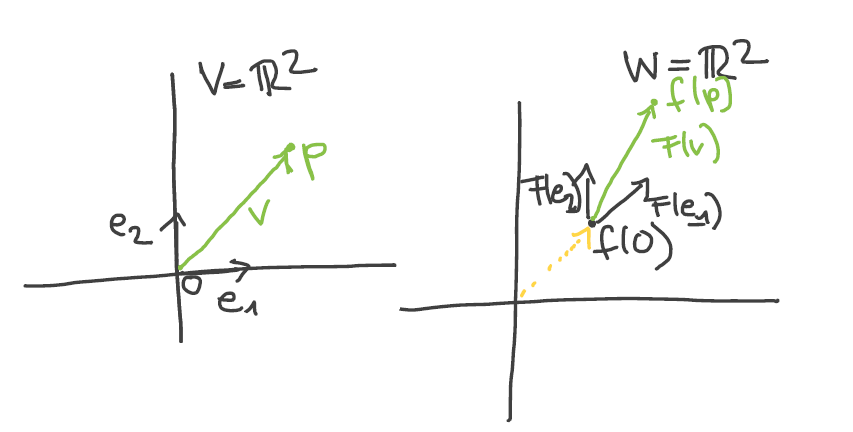
\includegraphics[width=0.7\linewidth]{figures/affine_abbildungen_vektorraeume}
    \label{fig:affine_abbildungen_vektorraeume}
\end{figure}
\begin{bemuebung*}
    Eine affine Abbildung \( f\maps X \to Y \) ist genau dann injektiv \bzw surjektiv \bzw bijektiv, wenn die zugehörige Abbildung \( F\maps T(X)\to T(Y) \) es ist.
\end{bemuebung*}
\begin{definition*}
    Wir nennen eine bijektive affine Abbildung \( f\maps X \to Y \) eine Affinität.
\end{definition*}
\subsection*{Affine Unterräume}
\begin{beispiel*}[\( \reals^2 \) als Vektorraum.]
    Untervektorräume von \( \reals^2 \) sind \( \emptyset \), \( \zeroset \), \( \reals^2 \) und Geraden durch \( 0 \).
    \begin{figure}[H]
        \centering
        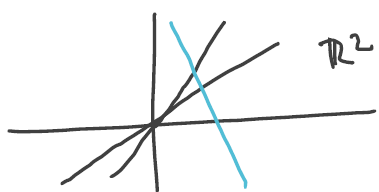
\includegraphics[width=0.4\linewidth]{figures/untervektorraeume_r2}
        \label{fig:untervektorraeume_r2}
    \end{figure}
    Betrachte nun \( \reals^2 \) als affinen Raum.
    \begin{figure}[H]
        \centering
        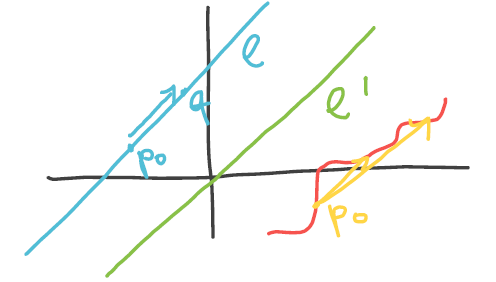
\includegraphics[width=0.5\linewidth]{figures/affine_unterraeume_r2}
        \label{fig:affine_unterraeume_r2}
    \end{figure}
    \begin{idee*}
        Wir wollen \( l \) und \( l' \) als affine Unterräume von \( \reals^2 \) definieren, da die Verschiebung von \( l, l' \) jeweils Untervektorräume von \( \reals^2 \) sind.
    \end{idee*}
\end{beispiel*}

\begin{definition*}
    Sei \( (X,T(X), \tau) \) in affiner Raum und \( Y\subseteq X \). Wenn es einen Punkt \( p_0 \in Y \) gibt, sodass
    \begin{align*}
        T(Y)\definedas \Set{\vv{p_0 q}\in T(X), q\in Y}
    \end{align*}
    ein Untervektorraum von \( T(X) \) ist, dann nennen wir \( Y \) einen affinen Unterraum von \( X \).
\end{definition*}
\begin{lemma}
    Sei \( Y\subseteq X \) ein affiner Unterraum eines affinen Raumes \( (X,T(X),\tau) \). Dann gilt
    \begin{align*}
        T(Y)=\Set{\vv{pq}\in T(X), q\in Y}
    \end{align*}
    für jeden beliebigen Punkt \( p\in Y \).
\end{lemma}
\begin{proof}
    Sei \( p_0\in Y \) ein fester Punkt mit
    \begin{align*}
        T(Y)=\Set{\vv{p_0 q}\in T(X), q \in Y}
    \end{align*}
    Untervektorraum von \( T(X) \).
    Dann gilt für \( p \in Y \)
    \begin{align*}
        \Set{\vv{pq}|q\in Y}=\vv{pp_0}+\Set{\vv{p_0 q}| q\in Y}=\underrelate{\textcolor{LimeGreen}{\vertni}}{\textcolor{LimeGreen}{T(Y)}}{\vv{p p_0}}+ T(Y)\textcolor{LimeGreen}{=T(Y)},
    \end{align*}
    \textcolor{LimeGreen}{da \( \vv{p p_0}=-\vv{p_0 p}\in T(Y) \)}.
    
\end{proof}
\begin{definition*}
    Sei \( Y\subseteq X \) ein affiner Unterraum. Wir nennen \( \dim-{K}{T(Y)} \) die Dimension von \( Y \) und schreiben 
    \begin{align*}
        \affindim-{Y}=\dim-{K}{T(Y)}.
    \end{align*}
\end{definition*}